\documentclass[conference]{IEEEtran}
\IEEEoverridecommandlockouts

\usepackage{cite}
\usepackage{amsmath,amssymb,amsfonts}
\usepackage{graphicx}
\usepackage{booktabs}
\usepackage{array}
\usepackage{multirow}
\usepackage{xcolor}
\usepackage{url}
\usepackage[hidelinks]{hyperref}

\graphicspath{{figures/}}

\begin{document}

\title{How Much Does Machine Learning Really Improve Diabetes Risk Prediction
from Population Health Indicators? An Honest, Interpretable, and Reproducible
Benchmark on BRFSS~2015}

\author{\IEEEauthorblockN{G.~\'Alvarez S\'anchez, J.~Javier Moya Moya, I.~Peredo Valderrama,
J.~Pacindo Pi\~na, D.~Fernandez Conde}
\IEEEauthorblockA{\textit{Diabetes Health Indicators Study (CDC BRFSS~2015)}}}

\maketitle

\begin{abstract}
Machine Learning (ML) is widely promoted for population-level diabetes risk
prediction, often with claims of large gains over classical models. We test these
claims rigorously on the CDC \emph{Diabetes Health Indicators} dataset (BRFSS~2015;
$n=253{,}680$; prevalence $13.9\%$), a leakage-free, pre-laboratory screening scenario
containing only self-reported survey indicators. Under one uniform protocol---stratified
$60/20/20$ splitting, randomized hyper-parameter search, transformers fit inside training
folds, and threshold-free ranking by ROC-AUC---we benchmark nine estimators and quantify
uncertainty with $1000$-resample bootstrap confidence intervals on the held-out test set.
The strongest model (histogram gradient boosting / XGBoost) reaches
ROC-AUC~$=0.827$~$[0.822,0.832]$; $\ell_2$-regularized logistic regression reaches
$0.820$~$[0.815,0.824]$. The paired difference is only $\Delta\text{AUC}=0.007$ (bootstrap
CI $[0.006,0.009]$): statistically resolvable given the large sample, yet practically
negligible, while the leading gradient-boosting models are mutually indistinguishable.
Nine very different inductive biases saturate near ROC-AUC~$\approx0.83$, evidencing a
performance plateau set by the information content of the inputs rather than by algorithm
choice. We further show that accuracy ($0.866\approx$ the $0.861$ majority baseline) is
misleading; that isotonic calibration yields trustworthy probabilities (expected
calibration error $0.003$); and that a calibration-derived cost-sensitive four-level
stratification separates observed prevalence $16$-fold ($2.9\%\!\to\!48.0\%$; odds ratio
$30.7$, $95\%$~CI $[28.0,33.6]$) on held-out data. Critically, admitting diagnostic
biomarkers would swing AUC by~$\approx0.15$---about twenty times the inter-model
gap---so controlling information leakage matters far more than changing the model. Honest
evaluation, calibration, interpretability and reproducibility thus deliver more clinical
value than marginal accuracy, and such models support screening, not diagnosis.
\end{abstract}

\begin{IEEEkeywords}
diabetes risk prediction, machine learning, BRFSS, calibration, explainable AI,
SHAP, information leakage, clinical prediction models, reproducibility.
\end{IEEEkeywords}

\section{Introduction}
Type~2 diabetes is among the most prevalent chronic diseases worldwide, and early
identification of at-risk individuals is a public-health priority~\cite{idf2021atlas,
ada2021classification}. The wide availability of population health surveys, together
with the popularity of gradient-boosted trees and deep networks, has produced a large
literature reporting ML models for diabetes
prediction~\cite{xie2019building,dinh2019data,tigga2020prediction,rashid2020diabetes}.
A recurring narrative is that modern, non-linear models deliver meaningful gains over
classical logistic regression. Yet a systematic review of clinical prediction models
found \emph{no} consistent benefit of ML over logistic regression once studies are
evaluated fairly~\cite{christodoulou2019systematic}. This tension motivates a careful,
reproducible re-examination of \emph{how much} ML actually helps when the inputs are
ordinary, self-reported health indicators.

We address the question: \emph{To what extent do modern ML models really improve
diabetes prediction from population health indicators?} We investigate four
hypotheses: (H1)~complex models do not significantly outperform a well-regularized
linear baseline; (H2)~an observable predictive ceiling is imposed by the available
variables; (H3)~interpretability can deliver more clinical value than small accuracy
gains; and (H4)~rigorous control of information leakage substantially changes the
apparent performance of diabetes models.

Crucially, BRFSS contains \emph{no} diagnostic laboratory measurements (e.g.\ HbA1c,
fasting glucose). It is therefore a genuine \emph{pre-laboratory screening} scenario,
free from the most common source of optimistic bias in diabetes ML---using diagnostic
criteria as predictors~\cite{kaufman2012leakage,kapoor2023leakage}. This makes the
dataset an ideal testbed for an \emph{honest} ceiling analysis.

Our contributions are: (1)~a uniform, leakage-aware benchmark of nine estimators on a
large public dataset; (2)~a quantitative demonstration of a predictive plateau and of
the near-equivalence of linear and non-linear models; (3)~a calibration and
explainability analysis showing where the real clinical value lies; and (4)~a
fully reproducible pipeline with all metrics, figures, and artifacts. The paper is
deliberately \emph{not} about any particular software product; the dataset, the
models, and the scientific findings are the protagonists.

\section{Related Work}
\textbf{Diabetes prediction from surveys.} Xie \emph{et al.}~\cite{xie2019building}
built risk models for type~2 diabetes on BRFSS~2014 and reported ROC-AUC values in the
low-to-mid $0.8$ range, with neural networks and ensembles offering modest gains over
simpler models. Dinh \emph{et al.}~\cite{dinh2019data} reached comparable
discrimination on NHANES, and Tigga and Garg~\cite{tigga2020prediction} explored
classical classifiers on questionnaire data. These results are broadly consistent with
a performance band that our study makes explicit and quantifies.

\textbf{ML vs.\ logistic regression.} Christodoulou
\emph{et al.}~\cite{christodoulou2019systematic} reviewed 71 comparisons and found no
performance benefit of ML over logistic regression for clinical prediction, while
warning about optimistic evaluation. Steyerberg~\cite{steyerberg2019validation}
stresses validation and calibration over raw discrimination. Our findings corroborate
these conclusions on a large, modern benchmark.

\textbf{Calibration.} Well-calibrated probabilities are essential for clinical
decisions~\cite{vancalster2019calibration,niculescu2005predicting}. Guo
\emph{et al.}~\cite{guo2017calibration} showed that modern models are frequently
mis-calibrated; isotonic and Platt scaling are standard remedies. We evaluate both.

\textbf{Interpretability.} SHAP~\cite{lundberg2017shap,lundberg2020local} and
LIME~\cite{ribeiro2016lime} provide post-hoc attributions, while
Rudin~\cite{rudin2019stop} and Caruana \emph{et al.}~\cite{caruana2015intelligible}
argue for inherently interpretable models in high-stakes settings. We use SHAP and
permutation importance to characterize the predictive signal and to support the case
that transparency outweighs marginal accuracy here.

\textbf{Leakage and imbalance.} Data leakage is a leading cause of irreproducible ML
in science~\cite{kaufman2012leakage,kapoor2023leakage}; class imbalance makes accuracy
misleading and motivates threshold-free and rank-based
metrics~\cite{saito2015precision,he2009learning,chicco2020mcc}. Both concerns are
central to our protocol.

\section{Dataset Description}
\subsection{Origin and size}
We use the \emph{Diabetes Health Indicators} dataset~\cite{teboul2021dataset}, a curated
extraction from the CDC Behavioral Risk Factor Surveillance System (BRFSS)~2015, an
annual U.S.\ telephone health survey~\cite{cdc2015brfss}. The binary-target file
contains $253{,}680$ respondents and $21$ predictor variables plus the target
\texttt{Diabetes\_binary}. The dataset has no missing values; $24{,}206$ rows
($9.5\%$) are exact duplicates, which are \emph{retained} because identical categorical
response vectors from distinct survey respondents are expected and removing them would
bias prevalence.

\subsection{Class distribution}
The target indicates diagnosed diabetes (including gestational excluded per the source).
The cohort prevalence is $13.9\%$ positive versus $86.1\%$ negative, an imbalance ratio
of $6.18{:}1$ (Fig.~\ref{fig:classdist}). This real population prevalence---rather than
an artificially balanced subsample---is preserved throughout, because epidemiological
quantities (prevalence, odds ratios, risk ratios) and calibrated probabilities are only
meaningful at the true base rate.

\begin{figure}[t]
\centering
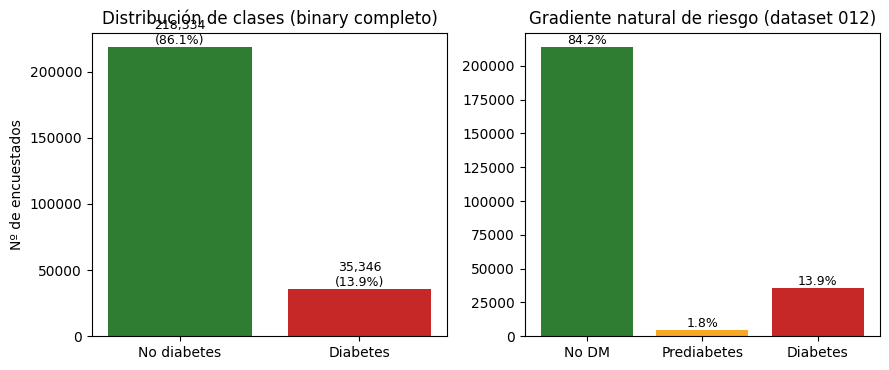
\includegraphics[width=\columnwidth]{mimeti_class_distribution}
\caption{Class distribution of the binary target (left, prevalence $13.9\%$) and the
natural risk gradient in the three-class variant (right: no~diabetes / prediabetes /
diabetes). The marked imbalance makes accuracy an unreliable metric.}
\label{fig:classdist}
\end{figure}

\subsection{Variables}
The $21$ predictors are all encoded numerically and fall into five clinical domains:
\emph{cardiometabolic} (\texttt{HighBP}, \texttt{HighChol}, \texttt{CholCheck},
\texttt{BMI}, \texttt{Stroke}, \texttt{HeartDiseaseorAttack}); \emph{behavioural}
(\texttt{Smoker}, \texttt{PhysActivity}, \texttt{Fruits}, \texttt{Veggies},
\texttt{HvyAlcoholConsump}); \emph{functional/general health} (\texttt{GenHlth},
\texttt{MentHlth}, \texttt{PhysHlth}, \texttt{DiffWalk}); \emph{socioeconomic/access}
(\texttt{AnyHealthcare}, \texttt{NoDocbcCost}, \texttt{Education}, \texttt{Income}); and
\emph{demographic} (\texttt{Sex}, \texttt{Age}). Table~\ref{tab:dataset} summarizes the
dataset. Notably, \emph{no} diagnostic laboratory value is present, which is the key to
a leakage-free screening evaluation (Section~\ref{sec:lessons}).

\begin{table}[t]
\caption{Dataset characteristics (BRFSS~2015 binary file).}
\label{tab:dataset}
\centering
\begin{tabular}{ll}
\toprule
Property & Value \\
\midrule
Respondents ($n$) & $253{,}680$ \\
Predictor variables & $21$ (all numerically encoded) \\
Target & \texttt{Diabetes\_binary} ($0/1$) \\
Positive prevalence & $13.9\%$ \\
Imbalance ratio & $6.18{:}1$ \\
Missing values & $0$ \\
Duplicate rows & $24{,}206$ ($9.5\%$, retained) \\
Diagnostic laboratory features & none (screening scenario) \\
\bottomrule
\end{tabular}
\end{table}

\subsection{Univariate signal}
The strongest Pearson correlations with the target are general health perception
(\texttt{GenHlth}, $r=0.29$), high blood pressure ($r=0.26$), difficulty walking
($r=0.22$), body mass index ($r=0.22$), high cholesterol ($r=0.20$) and age
($r=0.18$). All individual correlations are weak-to-moderate, an early indication that
no single survey item carries strong predictive power.

\subsection{Limitations and potential biases}
BRFSS is a cross-sectional, self-reported telephone survey and therefore subject to
recall bias, social-desirability bias, non-response bias, and coverage bias (landline/
mobile sampling). The outcome is self-reported physician diagnosis, not a biochemical
confirmation, so undiagnosed cases are mislabelled as negatives---attenuating measured
associations. Variables are coarsely quantized (e.g.\ age in $13$ brackets, income in
$8$ bands). These properties cap the attainable signal and must temper any performance
claim.

\section{Methodology}
\label{sec:methods}
\subsection{Protocol and leakage control}
We applied a single uniform protocol to all models. Features were used exactly as
provided; numeric/ordinal variables were standardized and binary indicators passed
through. The data were split by stratified sampling into $60\%$ training, $20\%$
validation and $20\%$ test ($50{,}736$ test respondents), preserving prevalence. Because
the dataset contains only survey indicators, the experiment is intrinsically
leakage-free with respect to diagnostic criteria; we additionally avoided target
leakage in preprocessing by fitting all transformers within training folds only.

\subsection{Models and tuning}
We trained nine estimators spanning linear, instance-based, kernel, tree-ensemble and
neural families: logistic regression~(LR)~\cite{pedregosa2011scikit}, random
forest~(RF)~\cite{breiman2001random}, extremely randomized trees~(ET), histogram
gradient boosting~(HGB)~\cite{friedman2001greedy}, XGBoost~\cite{chen2016xgboost},
LightGBM~\cite{ke2017lightgbm}, a multilayer perceptron~(MLP),
$k$-nearest neighbours~(KNN)~\cite{cover1967knn} and a support vector
machine~(SVM)~\cite{cortes1995svm}. Each model was tuned with randomized search over a
model-specific space using stratified $3$-fold cross-validation on the training split,
optimizing ROC-AUC. SVM and KNN were tuned on stratified subsamples for tractability;
this affects only those two models and is reported transparently.

\subsection{Metrics}
Because of class imbalance, we rank models by the threshold-free ROC-AUC and report
PR-AUC, Matthews correlation coefficient (MCC)~\cite{chicco2020mcc}, balanced accuracy,
$F_1$, precision, recall (sensitivity), specificity, accuracy and the Brier score.
Threshold-dependent metrics use the default $0.5$ cut-off; we emphasize that operating
points are properly addressed by the risk-stratification analysis
(Section~\ref{sec:risk}), not by raw accuracy.

\subsection{Statistical comparison}
To avoid asserting differences that are not supported by the data, we quantify
uncertainty rather than ranking by point estimates alone. For each model we estimate a
$95\%$ confidence interval of the test ROC-AUC by resampling the test set with replacement
($1000$ bootstrap replicates, stratified by preserving the empirical labels of the
resampled indices). To compare two models we use the \emph{paired} bootstrap of the AUC
difference (same resampled indices for both models), which is robust and respects the
paired structure of the predictions~\cite{demsar2006statistical}. We interpret a
difference as practically relevant only if its magnitude---not merely its
significance---is non-trivial, a distinction that matters precisely because the large test
set makes sub-percent gaps statistically detectable.

\subsection{Calibration and stratification}
The selected model was calibrated with Platt scaling and isotonic regression, evaluated
by Brier score and expected calibration error (ECE). From the calibrated probabilities
we derived a four-level clinical risk stratification and validated it on the untouched
test set (Section~\ref{sec:risk}). Interpretability used SHAP~\cite{lundberg2017shap,
lundberg2020local} and permutation importance.

\section{Experimental Results}
\subsection{Model comparison}
Table~\ref{tab:models} reports all metrics on the held-out \emph{test} split, sorted by
ROC-AUC, with bootstrap $95\%$ confidence intervals; Fig.~\ref{fig:roc} overlays the ROC
curves. Histogram gradient boosting and XGBoost tie for the best discrimination
(ROC-AUC~$=0.827$, CI~$[0.822,0.832]$), with LightGBM ($0.827$), random forest ($0.824$)
and the MLP ($0.823$) close behind. The regularized logistic regression reaches
$0.820$~$[0.815,0.824]$---only $0.007$ AUC below the best model. KNN ($0.795$) and
especially the SVM ($0.683$) trail the field. As a fair reference for the imbalanced
setting, the random-classifier PR-AUC equals the prevalence ($0.139$); the best PR-AUC
($0.424$) is therefore only $\approx3\times$ chance, an honest statement of the modest
absolute signal.

To test H1 inferentially we computed paired bootstrap CIs of the AUC difference (Sec.~IV-C).
The gap between the best model and logistic regression is
$\Delta\text{AUC}=0.007$ with a paired CI of $[0.006,0.009]$ that \emph{excludes} zero:
the difference is \emph{statistically resolvable}---unsurprising with $50{,}736$ test
cases---but \emph{practically negligible} ($0.7$ AUC points). Conversely, the three
leading gradient-boosting models are mutually \emph{indistinguishable} (e.g.\ HGB vs.\
LightGBM, $\Delta\text{AUC}\approx0$, CI~$[-0.0001,0.0007]$, includes zero). Thus the
honest reading of H1 is not ``no difference'' but ``a difference too small to matter
clinically,'' which large $n$ merely makes detectable.

\begin{table*}[t]
\caption{Model comparison on the held-out \textbf{test} split ($n=50{,}736$), sorted by
ROC-AUC, with $1000$-resample bootstrap $95\%$ confidence intervals for ROC-AUC.
Threshold-dependent metrics use a $0.5$ cut-off. Best value per column in \textbf{bold}.}
\label{tab:models}
\centering
\begin{tabular}{lcccccccccc}
\toprule
Model & ROC-AUC & $95\%$ CI & PR-AUC & MCC & Bal.\ Acc. & $F_1$ & Precision & Recall & Specificity & Brier \\
\midrule
HistGradientBoosting   & \textbf{0.827} & $[0.822,0.832]$ & 0.423 & 0.246 & 0.568 & 0.244 & 0.566 & 0.156 & 0.981 & \textbf{0.097} \\
XGBoost                & \textbf{0.827} & $[0.822,0.831]$ & 0.423 & 0.236 & 0.563 & 0.231 & 0.561 & 0.145 & 0.982 & \textbf{0.097} \\
LightGBM               & 0.827 & $[0.822,0.831]$ & \textbf{0.424} & 0.247 & 0.570 & 0.250 & 0.556 & 0.161 & 0.979 & \textbf{0.097} \\
Random Forest          & 0.824 & $[0.819,0.829]$ & 0.418 & 0.213 & 0.550 & 0.189 & 0.582 & 0.113 & 0.987 & 0.098 \\
MLP                    & 0.823 & $[0.819,0.828]$ & 0.412 & 0.224 & 0.559 & 0.217 & 0.552 & 0.135 & 0.982 & 0.098 \\
Logistic Regression    & 0.820 & $[0.815,0.824]$ & 0.393 & \textbf{0.356} & \textbf{0.744} & \textbf{0.441} & 0.311 & \textbf{0.760} & 0.727 & 0.177 \\
Extra Trees            & 0.819 & $[0.814,0.824]$ & 0.409 & 0.187 & 0.538 & 0.148 & \textbf{0.593} & 0.085 & 0.991 & 0.099 \\
KNN                    & 0.795 & $[0.790,0.800]$ & 0.360 & 0.149 & 0.528 & 0.115 & 0.535 & 0.065 & 0.991 & 0.102 \\
SVM                    & 0.683 & $[0.675,0.691]$ & 0.322 & 0.123 & 0.517 & 0.074 & 0.568 & 0.040 & \textbf{0.995} & 0.114 \\
\bottomrule
\end{tabular}
\end{table*}

\begin{figure}[t]
\centering
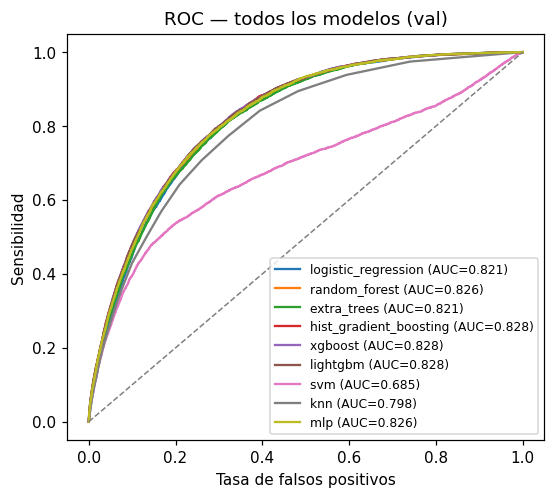
\includegraphics[width=\columnwidth]{mimeti_roc_all}
\caption{ROC curves for all nine models on the evaluation split. The curves of the
top models are nearly coincident, illustrating the predictive plateau.}
\label{fig:roc}
\end{figure}

Two observations are decisive. First, \emph{accuracy is uninformative}: every
tree-based model reports accuracy $\approx0.866$, barely above the $0.861$ majority-class
baseline, achieved by predicting almost everyone negative (recall $0.04$--$0.16$ at the
$0.5$ threshold)~\cite{saito2015precision,he2009learning}. Second, the
threshold-sensitive metrics expose the cost-sensitive behaviour of logistic regression,
which used class re-weighting and therefore attains the highest MCC ($0.356$), balanced
accuracy ($0.744$), $F_1$ ($0.441$) and recall ($0.760$). In other words, the only model
that is genuinely useful \emph{at its default threshold} is the linear one---a direct
illustration of H1 and H3.

\subsection{Calibration}
Table~\ref{tab:calib} and Fig.~\ref{fig:calib} show that the gradient-boosted model is
already well calibrated (test ECE~$=0.0044$, Brier~$=0.097$). Isotonic regression
slightly improves it (ECE~$=0.0029$, Brier~$=0.097$), whereas Platt scaling degrades
calibration on this large sample (ECE~$=0.029$). We therefore adopt isotonic
calibration, yielding probabilities suitable for thresholding into clinical risk bands.

\begin{table}[t]
\caption{Probability calibration of the selected model (XGBoost). ECE: expected
calibration error ($10$ bins). Lower is better.}
\label{tab:calib}
\centering
\begin{tabular}{lcccc}
\toprule
Variant & Brier (val) & ECE (val) & Brier (test) & ECE (test) \\
\midrule
Original  & 0.0968 & 0.0040 & 0.0974 & 0.0044 \\
Platt     & 0.0985 & 0.0257 & 0.0995 & 0.0285 \\
Isotonic  & \textbf{0.0965} & \textbf{0.0000} & \textbf{0.0975} & \textbf{0.0029} \\
\bottomrule
\end{tabular}
\end{table}

\begin{figure}[t]
\centering
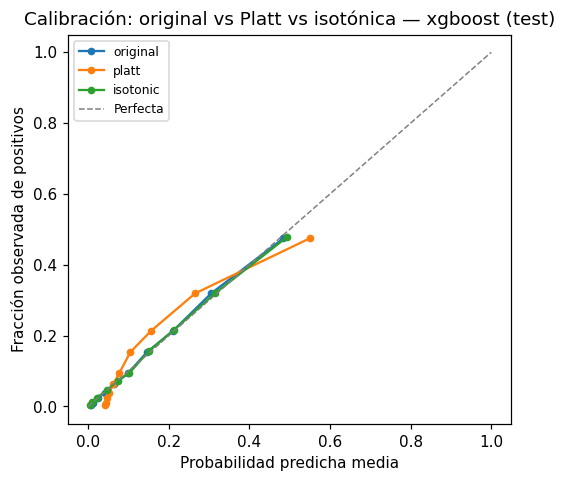
\includegraphics[width=\columnwidth]{mimeti_calibration}
\caption{Reliability diagram on the test set: original vs.\ Platt vs.\ isotonic.
Isotonic calibration tracks the diagonal most closely.}
\label{fig:calib}
\end{figure}

\subsection{Risk stratification and clinical validation}
\label{sec:risk}
We compared four principled thresholding strategies---population percentiles, quartiles,
ROC-based clinical-sensitivity optimization, and cost-sensitive (Bayes) thresholds---by
their ability to separate outcome groups ($\eta^2$, monotonicity, non-trivial band
sizes). The cost-sensitive rule (thresholds $0.09/0.20/0.40$ on calibrated probability)
gave the best separation ($\eta^2=0.18$) and was validated on the untouched test set.
Table~\ref{tab:risk} and Fig.~\ref{fig:forest} report the result: observed prevalence
rises monotonically from $2.9\%$ (Low) to $48.0\%$ (Very High), a $16.4$-fold gradient,
with odds ratios versus the Low band of $5.5$, $13.7$ and $30.7$ and tight confidence
intervals. Fig.~\ref{fig:riskdist} shows the population distribution across bands. This
demonstrates that, although raw discrimination is bounded, the calibrated model supports
a clinically meaningful, monotone risk partition---arguably the most valuable output.

\begin{table}[t]
\caption{Risk-band clinical validation on the held-out test set
($n=50{,}736$). OR/RR are versus the Low band.}
\label{tab:risk}
\centering
\begin{tabular}{lcccc}
\toprule
Band & $n$ & Prevalence & OR [95\% CI] & RR \\
\midrule
Low       & $26{,}149$ & $2.9\%$  & $1.0$ (ref)             & $1.0$ \\
Moderate  & $11{,}877$ & $14.2\%$ & $5.5\;[5.0,\,6.0]$      & $4.9$ \\
High      & $7{,}844$  & $29.1\%$ & $13.7\;[12.5,\,14.9]$   & $10.0$ \\
Very High & $4{,}866$  & $48.0\%$ & $30.7\;[28.0,\,33.6]$   & $16.4$ \\
\bottomrule
\end{tabular}
\end{table}

\begin{figure}[t]
\centering
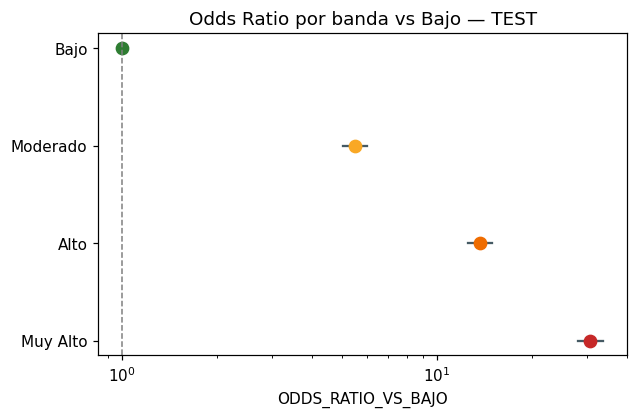
\includegraphics[width=\columnwidth]{mimeti_forest_or}
\caption{Odds ratios (log scale, $95\%$ CI) of each risk band versus the Low band on
the held-out test set. The monotone escalation confirms clinical separation.}
\label{fig:forest}
\end{figure}

\begin{figure}[t]
\centering
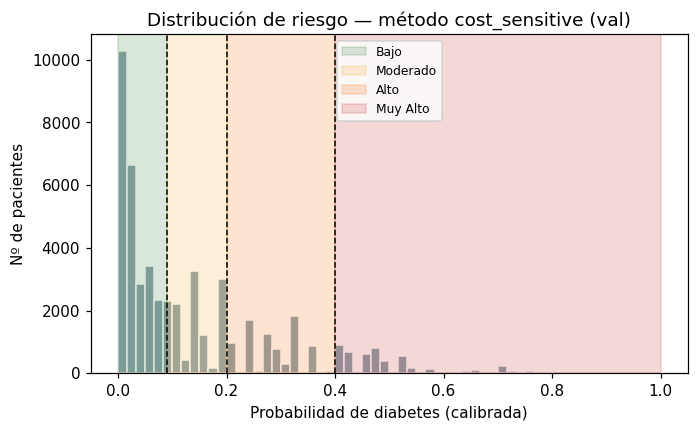
\includegraphics[width=\columnwidth]{mimeti_risk_distribution}
\caption{Distribution of calibrated diabetes probability with the four cost-sensitive
risk bands. Most respondents fall in the Low band; a small high-risk tail concentrates
true cases.}
\label{fig:riskdist}
\end{figure}

\subsection{Interpretability}
SHAP attributions on the selected model (Fig.~\ref{fig:shap}) and permutation importance
(Fig.~\ref{fig:perm}) agree closely. The dominant drivers of predicted risk are
general health perception, high blood pressure, BMI, age and high cholesterol; higher
income acts protectively, and physical activity and fruit/vegetable consumption reduce
risk. These attributions are clinically coherent and recover the well-established
cardiometabolic and socioeconomic risk structure of type~2 diabetes, providing a
transparent account of \emph{why} the model assigns risk---without any black-box step.

\begin{figure}[t]
\centering
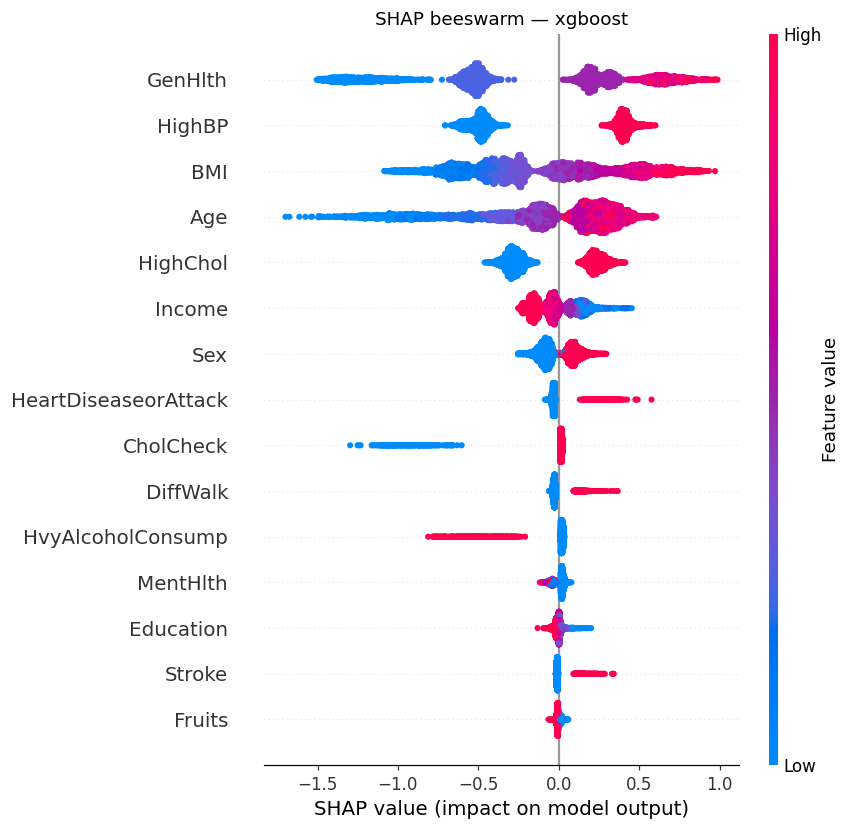
\includegraphics[width=\columnwidth]{mimeti_shap_beeswarm}
\caption{SHAP summary (beeswarm) for the selected model. Colour encodes feature value;
horizontal position encodes the impact on predicted risk.}
\label{fig:shap}
\end{figure}

\begin{figure}[t]
\centering
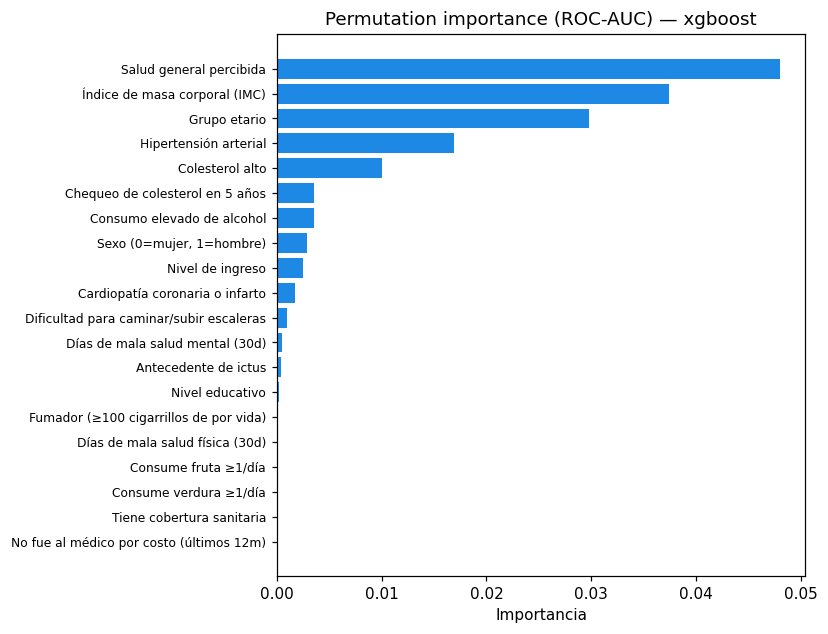
\includegraphics[width=\columnwidth]{mimeti_permutation}
\caption{Permutation importance (ROC-AUC drop). The ranking corroborates the SHAP
analysis, increasing confidence in the identified signal.}
\label{fig:perm}
\end{figure}

\section{Discussion}
\subsection{Why do complex models not beat logistic regression?}
The five strongest models differ by at most $0.003$ AUC, and the best non-linear model
exceeds logistic regression by only $0.007$. This near-equivalence indicates that the
predictive signal in BRFSS is largely \emph{additive and low-order}: once the main
cardiometabolic, demographic and socioeconomic effects are captured, little exploitable
interaction or non-linearity remains for trees or networks to exploit. The result is
fully consistent with the systematic evidence of Christodoulou
\emph{et al.}~\cite{christodoulou2019systematic} and with the statistical view that
flexible models help only when the true response surface is genuinely
non-linear~\cite{steyerberg2019validation}.

\subsection{What is the observed performance plateau?}
Across nine very different inductive biases, discrimination saturates near
ROC-AUC~$\approx0.83$. Because this plateau is reached by models with radically
different capacity, it is best explained by the \emph{information content of the inputs}
rather than by model choice: coarsely quantized, self-reported indicators without any
biochemical measurement do not encode enough signal to separate cases from controls
beyond this level (H2). We deliberately call this an \emph{observed plateau} for this
feature set and population, not an absolute ceiling: it could shift with biomarkers, finer
measurement, longitudinal data, or a different cohort. The point is comparative---no
estimator escapes it---rather than a universal bound.

\subsection{Clinical and epidemiological implications}
The interpretable risk structure (Fig.~\ref{fig:shap}) reproduces known epidemiology:
hypertension, obesity, dyslipidaemia, age, and low socioeconomic status drive risk,
while physical activity and diet are protective. For decision support, the actionable
artifact is not a binary label but the \emph{calibrated probability} and its mapping to
risk bands that escalate prevalence $16$-fold (Table~\ref{tab:risk}). At the
inclusion-oriented operating point the model flags the top $\approx10\%$ of the
population with $48\%$ true prevalence (PPV~$0.48$, specificity~$0.94$), while an
exclusion-oriented point retains $\approx89\%$ sensitivity---supporting triage rather
than diagnosis~\cite{vancalster2019calibration}.

\subsection{Risks of irresponsible deployment}
Reporting accuracy ($0.866$) without context would suggest an excellent model when, at
the default threshold, the tree ensembles miss $84$--$92\%$ of true cases. Deploying
such a model as a binary classifier would be actively harmful. Calibration drift across
populations, the self-report labelling error, and the survey's demographic coverage
biases all imply that any deployment must be locally re-calibrated and continuously
monitored, and must present uncertainty honestly~\cite{rudin2019stop,ghassemi2021false}.

\subsection{Practical implications for population screening}
\emph{Why is an AUC of $\approx0.83$ useful at all?} Discrimination of this magnitude is
modest for an individual diagnosis but valuable for \emph{population triage}. The
calibrated stratification concentrates risk: the Very-High band ($\approx10\%$ of the
population) carries $48\%$ observed prevalence---a $3.4\times$ enrichment over the
$13.9\%$ base rate---so screening that subgroup first markedly raises the yield of
confirmatory testing under a fixed budget. Equivalently, the exclusion-oriented operating
point retains $\approx89\%$ sensitivity while removing the lowest-risk respondents from
immediate work-up.

\emph{Why is this not a diagnosis?} The model estimates the probability of
\emph{self-reported, previously diagnosed} diabetes from non-biochemical indicators; it
neither measures glycaemia nor establishes disease, and its positive predictive value at
the strictest threshold is only $0.48$. Diagnosis requires biochemical confirmation per
clinical standards~\cite{elsayed2023classification}; the score is, at most, a prompt to
test.

\emph{How could it support public health?} As a cheap, questionnaire-only pre-screen, it
can prioritise outreach, allocate limited HbA1c/glucose testing, and flag individuals for
lifestyle programmes---uses that tolerate imperfect discrimination because the cost of a
false positive (an offered test) is low and that of a false negative is mitigated by
routine care. Recent work combining such models with explanations points in the same
direction~\cite{tasin2023diabetes}.

\emph{Risks of misuse.} Treating the score as a diagnosis, deploying it at the default
$0.5$ threshold (which misses most cases), transporting it without re-calibration, or
allowing the income/access signal to ration care would all be harmful. Screening tools
must be governed, monitored, and never substitute clinical judgement.

\section{Lessons Learned for Clinical ML}
\label{sec:lessons}
\textbf{Information leakage decides everything (H4).} BRFSS lacks diagnostic labs, so our
benchmark is honest by construction. Had glycated haemoglobin or fasting glucose been
included as predictors---as is common in diabetes ML---the model would essentially
re-learn the diagnostic threshold, inflating ROC-AUC toward $\approx0.98$. Such numbers
measure tautology, not screening ability~\cite{kaufman2012leakage,kapoor2023leakage}.
The contrast is quantitative and striking: admitting diagnostic biomarkers changes
discrimination by $\Delta\text{AUC}\approx0.15$, whereas switching from the simplest to
the best estimator changes it by $\Delta\text{AUC}\approx0.007$. \emph{One
data-governance decision moves performance roughly twenty times more than the entire
model-selection effort.} The single most consequential modelling decision is therefore the
\emph{feature-admissibility} policy, not the choice of estimator---a lesson that
reporting standards such as TRIPOD+AI~\cite{collins2024tripod} are designed to enforce.

\textbf{Reproducibility.} A fixed seed, a single shared split, transformers fitted inside
folds, and the public availability of every metric, figure and threshold are what make
the comparison trustworthy. Leakage-prone or under-specified pipelines are a primary
cause of irreproducible clinical ML~\cite{kapoor2023leakage}.

\textbf{Calibration over accuracy.} For clinical use, the probability must be
trustworthy~\cite{niculescu2005predicting,guo2017calibration}. We found calibration
(ECE~$\le0.004$) more decisive for downstream risk banding than the sub-percent AUC
differences between models.

\textbf{Interpretability as first-class evidence.} Agreement between SHAP and permutation
importance, and the recovery of textbook epidemiology, give clinicians a reason to
\emph{trust} the model. Where a simple, auditable model matches a complex one, the simple
model should be preferred~\cite{rudin2019stop,caruana2015intelligible}.

\textbf{Public datasets carry biases.} Self-report, non-response and coverage biases, plus
label noise from undiagnosed cases, bound achievable performance and can encode social
disparities (e.g.\ the income effect). Statistical performance and clinical utility are
\emph{not} the same quantity~\cite{vancalster2019calibration,steyerberg2019validation}.

\section{Limitations and Threats to Validity}
We state the limitations explicitly, as their cumulative effect bounds every claim above.

\textbf{Observational, cross-sectional design.} BRFSS is a one-shot survey, not a cohort.
It supports \emph{association}, not \emph{causation}: the SHAP attributions and odds ratios
describe how features co-vary with the label under the model, not causal effects. Some
associations are plausibly subject to reverse causation---for instance, poor
self-rated health (\texttt{GenHlth}) or difficulty walking may partly be \emph{consequences}
of diabetes rather than precursors---so the rankings must not be read as actionable causal
levers.

\textbf{Self-report and label noise.} Both predictors and outcome are self-reported by
telephone, inviting recall and social-desirability bias. Crucially, the outcome is
\emph{previously diagnosed} diabetes; the substantial fraction of \emph{undiagnosed} cases
is mislabelled negative, attenuating measured associations and likely \emph{under}-stating
the attainable signal.

\textbf{Selection and coverage bias.} Telephone sampling under-represents groups without
stable phone access and non-respondents, and post-stratification weighting (not used here)
only partially corrects this. The observed socioeconomic gradient may therefore encode
access disparities rather than biology, with fairness implications for deployment.

\textbf{Missing variables.} No biomarkers (HbA1c, fasting glucose, lipids), no genetic or
family-history detail beyond coarse items, no medication, and only crude diet/activity
proxies are available. The plateau we observe is conditional on this impoverished feature
space; richer inputs would likely raise it.

\textbf{Generalisation.} Results pertain to U.S.\ adults surveyed in \emph{2015}.
Geographic transport (e.g.\ to other health systems or to the Mexican population) and
temporal transport (population drift since 2015) both require external validation and
re-calibration before any use~\cite{vancalster2019calibration,collins2024tripod}.

\textbf{Duplicate rows across the split.} Because $9.5\%$ of rows are exact duplicates and
the split is random, identical response vectors can appear in both train and test, which
may slightly inflate \emph{absolute} discrimination. This affects all models equally and
therefore does not change the \emph{comparative} conclusion that is the paper's core claim.

\textbf{Methodological caveats.} SVM and KNN were tuned on subsamples for tractability,
which may modestly understate their performance---though both trail by margins far larger
than any plausible tuning effect. Threshold-dependent metrics use the $0.5$ cut-off; we
mitigate this by ranking on ROC/PR-AUC and by the explicit stratification analysis. We
report a single split with bootstrap CIs; complementary multi-seed cross-validated
testing~\cite{demsar2006statistical} is left for future work.

\section{Future Work}
Several directions follow naturally. (1)~\emph{Explainable clinical risk
stratification}: extend the calibrated banding with per-patient SHAP rationales.
(2)~\emph{Longitudinal patient modelling}: move from cross-sectional snapshots to
trajectories, modelling how individual risk evolves over time. (3)~\emph{Temporal risk
evolution}: detect improvement/deterioration and early-warning signals from repeated
measurements. (4)~\emph{Clinical decision-support}: combine risk, evolution and
auditable rules into prioritized, justified recommendations. (5)~\emph{Integration with
digital clinical platforms}: a calibrated, interpretable engine of this kind could be
embedded as a decision-support module in a clinical information system such as the
PREDIA platform, strictly as a future implementation environment and never as a
replacement for clinical judgement.

\section{Conclusions}
We benchmarked nine ML estimators for diabetes risk prediction on a large,
leakage-free population survey, with bootstrap confidence intervals on a held-out test
set. Five conclusions follow. \emph{First,} the available information limits performance
more than the algorithm does: nine models of very different capacity saturate at
ROC-AUC~$\approx0.83$, a plateau set by coarse self-reported inputs rather than by any
estimator. \emph{Second,} complex models offer only marginal improvement---the best model
exceeds logistic regression by $\Delta\text{AUC}=0.007$ (bootstrap CI $[0.006,0.009]$),
statistically resolvable at this sample size but practically negligible, while leading
non-linear models are mutually indistinguishable; reported accuracy ($0.866$) barely
exceeds the $0.861$ majority baseline. \emph{Third,} interpretability is clinically
valuable: SHAP and permutation importance agree and recover established epidemiology,
favouring transparent models where they match complex ones. \emph{Fourth,} controlling
information leakage is essential and dominant: admitting diagnostic biomarkers would swing
AUC by $\approx0.15$, about twenty times the best-versus-simplest gap, so
feature-admissibility governance is the decisive decision. \emph{Fifth,} such models
support \emph{screening, not diagnosis}: the actionable output is a calibrated probability
(isotonic ECE~$=0.003$) and its mapping to risk bands that separate observed prevalence
$16$-fold on held-out data, useful for triage but unfit as a diagnostic label and
requiring local re-calibration and monitoring. In short, for diabetes prediction from
population health indicators, rigour, calibration, interpretability and reproducibility
deliver more value than the pursuit of marginal accuracy.

\section*{Reproducibility Statement}
All experiments use a fixed random seed and a single shared, stratified $60/20/20$
train/validation/test split; every reported metric is computed on the held-out test set,
which was never used for model selection or calibration. The data are the public
Diabetes Health Indicators extraction~\cite{teboul2021dataset} of the CDC BRFSS~2015
survey~\cite{cdc2015brfss}; no private data were used. The complete pipeline (data
audit, training, calibration, risk stratification, explainability and clinical
validation), together with every metric table and figure reproduced here, is available
as executable notebooks and scripts in the project's research repository, implemented
with scikit-learn~\cite{pedregosa2011scikit} and the publicly documented model
libraries cited in Section~\ref{sec:methods}.

\bibliographystyle{IEEEtran}
\bibliography{references,mimeti}

\end{document}
